\documentclass[11pt,a4paper]{article}
\usepackage[margin=1.0in]{geometry}
\usepackage{setspace}
\doublespacing
\usepackage{enumitem}
\usepackage{url}
%%%%%%%%%%%%%%%%%%%%%%%%%%%%%%%%%%%%%%%%%%%%%%%%%%%%%%%%%%%%%%%%
%% Graphicx.sty for Including PostScript .eps files
\usepackage{graphicx}
\usepackage{epstopdf}
\usepackage{caption}
%%%%%%%%%%%%%%%%%%%%%%%%%%%%%%%%%%%%%%%%%%%%%%%%%%%%%%%%%%%%%%%%

\makeatletter
    \setlength\@fptop{0\p@}
\makeatother

\begin{document}

%% Title Pages
%% Setting up title pages, type in the appropriate names here:
\title{Description of the FMCs and Corresponding Hardware for the 2CBC2 \\ version 0.00}

\author{Fionn Ball\\
	f.ball@cern.ch}
	%or
	%\authors{}

	\maketitle
	\tableofcontents

	\section{Introduction}
	This document will briefly describe the various iterations of the FMCs and firmware needed for the test stand. Both FMCs will work with the 2CBC2, however they require a different firmware and cable. The correct cable should have been provided with the FMC.
	
	\section{Old 2CBC2 FMC}
	Uses \verb|firmware/OLD_glib_be.bit|. See Fig.\ref{fig:OFMC} and Fig.\ref{fig:OCable}.
	
\begin{figure} [htbp] 
        \centering
                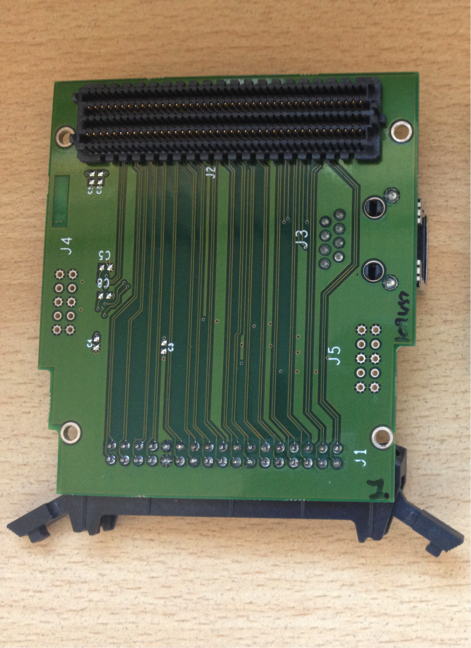
\includegraphics[width=0.5\textwidth]{fig/OLD_FMC.png}
                \caption{Old FMC. Notice connectors are on opposing sides.}
                \label{fig:OFMC}
        \end{figure}
        
\begin{figure}[htbp]
		\centering
                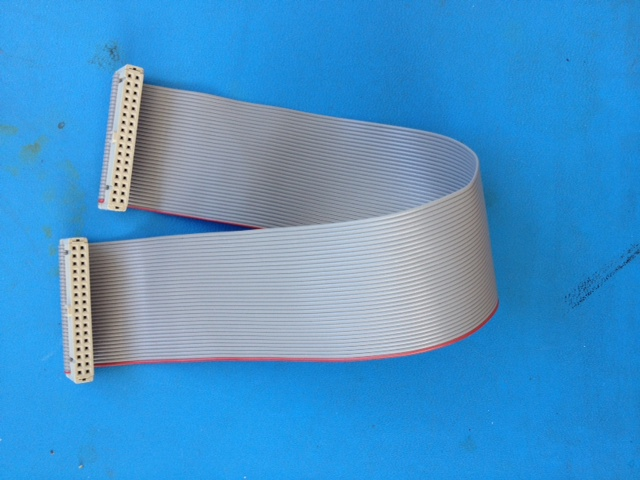
\includegraphics[width=0.5\textwidth, angle = 270]{fig/OldCable.png}
                \caption{Old cable. Cable is as standard.}
                \label{fig:OCable}
\end{figure}

	\section{New 2CBC2 FMC}
	
	Uses \verb|firmware/NEW_glib_be.bit|. See Fig.\ref{fig:NFMC} and Fig.\ref{fig:NCable}.	
	
\begin{figure} [htbp] 
        \centering
                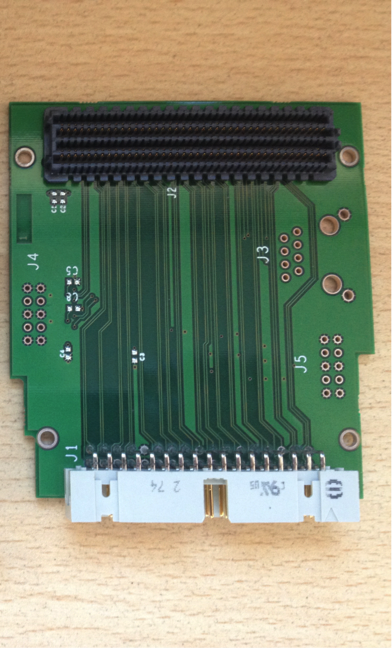
\includegraphics[width=0.5\textwidth]{fig/NEW_FMC.png}
                \caption{New FMC. Notice connectors are on same side.}
                \label{fig:NFMC}
\end{figure}

\begin{figure} [htbp] 
		\centering
                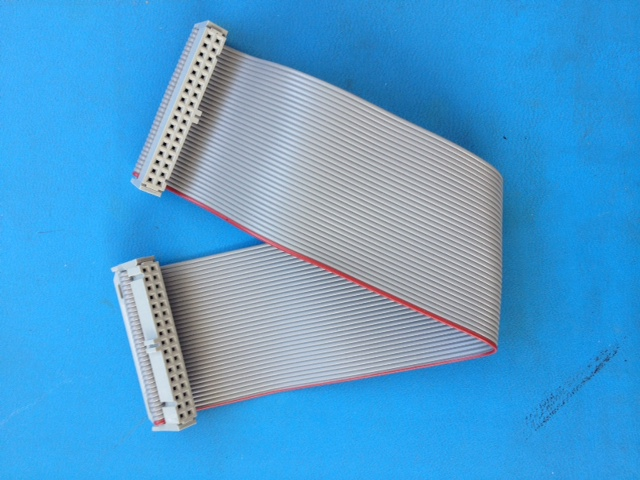
\includegraphics[width=0.5\textwidth, angle = 270]{fig/NewCable.png}
                \caption{New cable. Notice end connectors are flipped.}
                \label{fig:NCable}
        \end{figure}
        
	\end{document}

